
\de{ĐỀ THI ÔN TẬP  HỌC KỲ II NĂM HỌC 2022-2023}{THPT Tân Bình}
\begin{center}
	\textbf{PHẦN 1 - TRẮC NGHIỆM}
\end{center}

\Opensolutionfile{ans}[ans/ans]
\begin{ex}%[Dự án Tex đề HK2 2022-2023 L1]%[Nhật Thiện]%[0T9Y4-1]
	Trong mặt phẳng tọa độ $Oxy$, phương trình nào sau đây là phương trình chính tắc của Elip?
	\choice
	{\True $\dfrac{x^2}{100}+\dfrac{y^2}{64}=1$}
	{$\dfrac{x^2}{100}-\dfrac{y^2}{64}=0$}
	{$\dfrac{x^2}{100}-\dfrac{y^2}{64}=1$}
	{$\dfrac{x^2}{100}+\dfrac{y^2}{64}=0$}
\loigiai{
Phương trình $\dfrac{x^2}{100}+\dfrac{y^2}{64}=1$ là phương trình chính tắc của ELip.
}
\end{ex}
\begin{ex}%[Dự án Tex đề HK2 2022-2023 L1]%[Nhật Thiện]%[0T8Y2-1]
	Một tổ có $6$ học sinh nữ và $9$ học sinh nam. Hỏi có bao nhiêu cách chọn $2$ học sinh nam và $1$ học sinh nữ đi lao động
	\choice
	{$\mathrm{C}_6^2+\mathrm{C}_9^1$}
	{$\mathrm{C}_9^2+\mathrm{C}_6^1$}
	{$\mathrm{C}_6^2\cdot \mathrm{C}_9^1$}
	{\True $\mathrm{C}_9^2\cdot \mathrm{C}_6^1$}
\loigiai{
Bước 1. Chọn $2$ học sinh nam có $\mathrm{C}_9^2$ cách.\\
Bước 2. Chọn $1$ học sinh nữ có $\mathrm{C}_6^1$ cách.\\
Theo quy tắc nhân có $\mathrm{C}_9^2\cdot \mathrm{C}_6^1$ cách chọn thỏa mãn bài toán.
}
\end{ex}
\begin{ex}%[Dự án Tex đề HK2 2022-2023 L1]%[Nhật Thiện]%[0T9Y1-3]
	Trong mặt phẳng $Oxy$, cho tam giác $ABC$ với $A(2;-1)$, $B(0;6)$, $C(-5;1)$. Tọa độ trọng tâm của tam giác $ABC$ là
	\choice
	{$(1;2)$}
	{$(-1;-2)$}
	{$(1;-2)$}
	{\True $(-1;2)$}
\loigiai{
Giả sử $G$ là trọng tâm tam giác $ABC$, tọa độ trọng tâm $G$ thỏa
$$\heva{&x_G=\dfrac{x_A+x_B+x_C}{3}\\&y_G=\dfrac{y_A+y_B+y_C}{3}}\Leftrightarrow \heva{&x_G=\dfrac{2+0+(-5)}{3}=-1\\&y_G=\dfrac{(-1)+6+1}{3}=2.}$$
Vậy $G(-1;2)$.
}
\end{ex}
\begin{ex}%[Dự án Tex đề HK2 2022-2023 L1]%[Nhật Thiện]%[0T9Y3-1]
	Tọa độ tâm $I$ và bán kính $R$ của đường tròn $(C)\colon (x+1)^2+y^2=8$ là
	\choice
	{$I(1;0)$, $R=2\sqrt{2}$}
	{$I(-1;0)$, $R=8$}
	{$I(-1;0)$, $R=64$}
	{\True $I(-1;0)$, $R=2\sqrt{2}$}
\loigiai{
Đường tròn $(C)\colon (x+1)^2+y^2=8$ có tâm $I(-1;0)$ và bán kính $R=\sqrt{8}=2\sqrt{2}$.
}
\end{ex}
\begin{ex}%[Dự án Tex đề HK2 2022-2023 L1]%[Nhật Thiện]%[0T0Y2-2]
	Tung một con xúc xắc cân đối đồng chất. Tính xác suất để xuất hiện mặt có số chấm chẵn
	\choice
	{$\dfrac{1}{6}$}
	{$\dfrac{2}{3}$}
	{\True $\dfrac{1}{2}$}
	{$\dfrac{1}{3}$}
\loigiai{
$n(\Omega)=6$.\\
Gọi $A$ là biến cố ``xuất hiện số chấm chẵn''.\\
Suy ra $n(A)=3$.\\
Vậy $\mathrm{P}(A)=\dfrac{n(A)}{n(\Omega)}=\dfrac{3}{6}=\dfrac{1}{2}$.
}
\end{ex}
\begin{ex}%[Dự án Tex đề HK2 2022-2023 L1]%[Nhật Thiện]%[0T7B1-1]
	Tam thức bậc hai nào sau đây có bảng xét dấu như sau?
	\begin{center}
		
\begin{tikzpicture}[scale=1, font=\footnotesize, line join=round, line cap=round, >=stealth]
			\tkzTabInit[nocadre=false,lgt=1.2,espcl=2.5,deltacl=0.6]
			{$x$ /0.6,$f(x)$ /0.6}
			{$-\infty$,$-2$,$4$,$+\infty$}
			\tkzTabLine{,-,0,+,0,-,}
		\end{tikzpicture}
	\end{center}
	\choice
	{\True $f(x)=-x^2+2x+8$}
	{$f(x)=-x^2-6x+8$}
	{$f(x)=x^2+6x-8$}
	{$f(x)=x^2-2x-8$}
\loigiai{
Xét $f(x)=-x^2+2x+8$ có $\Delta=36>0$, hai nghiệm phân biệt là $x_1=-2$, $x_2=4$ và $a=-1<0$ nên ta có bảng xét dấu $f(x)$ như sau
\begin{center}
	
\begin{tikzpicture}[scale=1, font=\footnotesize, line join=round, line cap=round, >=stealth]
		\tkzTabInit[nocadre=false,lgt=1.2,espcl=2.5,deltacl=0.6]
		{$x$ /0.6,$f(x)$ /0.6}
		{$-\infty$,$-2$,$4$,$+\infty$}
		\tkzTabLine{,-,0,+,0,-,}
	\end{tikzpicture}
\end{center}
}
\end{ex}
\begin{ex}%[Dự án Tex đề HK2 2022-2023 L1]%[Nhật Thiện]%[0T8Y2-1]
	Từ các chữ số $1$, $2$, $3$, $4$, $5$ có thể lập được bao nhiêu số tự nhiên có $3$ chữ số đôi một khác nhau?
	\choice
	{$\dfrac{5!}{3!}$}
	{$5!$}
	{\True $\mathrm{A}_5^3$}
	{$\mathrm{C}_5^3$}
\loigiai{
Lập số tự nhiên có $3$ chữ số đôi một khác nhau có $\mathrm{A}_5^3$ cách.
}
\end{ex}
\begin{ex}%[Dự án Tex đề HK2 2022-2023 L1]%[Nhật Thiện]%[0T9Y4-4]
	Trong mặt phẳng tọa độ $Oxy$, phương trình nào sau đây là phương trình chính trắc của hypebol?
	\choice
	{$x^2+y^2=1$}
	{$\dfrac{x^2}{9}-\dfrac{y^2}{4}=0$}
	{\True $\dfrac{x^2}{9}-\dfrac{y^2}{4}=1$}
	{$y^2=9x$}
\loigiai{
Phương trình $\dfrac{x^2}{9}-\dfrac{y^2}{4}=1$ là phương trình chính tắc của hypebol.
}
\end{ex}
\begin{ex}%[Dự án Tex đề HK2 2022-2023 L1]%[Nhật Thiện]%[0T8Y2-1]
	Công thức tính số hoán vị $\mathrm{P}_n$ là
	\choice
	{$\mathrm{P}_n=(n-1)!$}
	{$\mathrm{P}_n=(n+1)!$}
	{\True $\mathrm{P}_n=n!$}
	{$\mathrm{P}_n=\dfrac{n!}{(n-k)!}$}
\loigiai{
Ta có $\mathrm{P}_n=n!$.
}
\end{ex}
\begin{ex}%[Dự án Tex đề HK2 2022-2023 L1]%[Nhật Thiện]%[0T8Y1-2]
	Bạn Lan có $3$ chiếc quần khác nhau và $4$ chiếc áo khác nhau. Bạn Lan muốn chọn ra $1$ bộ quần áo trong số đó. Hỏi bạn Lan có bao nhiêu cách chọn?
	\choice
	{$3$}
	{$4$}
	{$7$}
	{\True $12$}
\loigiai{
Bước 1. Chọn $1$ chiếc quần có $3$ cách.\\
Bước 2. Chọn $1$ chiếc áo có $4$ cách.\\
Theo quy tắc nhân, có $3\cdot 4=12$ cách chọn thỏa mãn.
}
\end{ex}

\begin{ex}%[Đề thi HK2, THPT Tân Bình-TPHCM]%BC Tuan%[0T8Y1-1]
	Một cửa hàng sách có bán $5$ loại bút bi khác nhau và $7$ loại bút máy khác nhau. Có bao nhiêu cách để một bạn học sinh mua $1$ loại bút từ cửa hàng?
		\choice{$14$}{$25$}{\True $12$}{$35$}
\loigiai{
Theo quy tắc cộng, số cách để một bạn học sinh mua $1$ loại bút từ cửa hàng là $5+7=12$.
}
\end{ex}
\begin{ex}%[Đề thi HK2, THPT Tân Bình-TPHCM]%BC Tuan%[0T8Y1-2]
Một người gieo đồng xu hai mặt, sau mỗi lần gieo thì kết quả nhận được luôn là sấp hoặc ngửa. Nếu người này gieo $5$ lần thì số kết quả có thể xảy ra là
\choice{$2$}{$10$}{$25$}{\True $32$}
\loigiai{
Mỗi lần gieo, có $2$ kết quả có thể xảy ra.\\
Theo quy tắc nhân, sau $5$ lần gieo, số kết quả có thể xảy ra là $2^5=32$.
}
\end{ex}
\begin{ex}%[Đề thi HK2, THPT Tân Bình-TPHCM]%BC Tuan%[0T9B3-2]
Trong các phương trình sau phương trình nào là phương trình của một đường tròn?
\choice{$x^2+2y^2+2x-4y+9=0$}
{\True $x^2+y^2-2x+8y-2=0$}
{$2x^2+y^2+2x-3y+9=0$}
{$x^3+y^2-6x+4y+13=0$}
\loigiai{
Phương trình $x^2+y^2-2ax-2by+c=0$ với $a^2+b^2-c>0$ là phương trình của một đường tròn.\\
Trong các đáp án trên, phương trình $x^2+y^2-2x+8y-2=0$ là phương trình của một đường tròn.
}
\end{ex}
\begin{ex}%[Đề thi HK2, THPT Tân Bình-TPHCM]%BC Tuan%[0T9Y2-2]
	Trong mặt phẳng $Oxy$, phương trình tham số của đường thẳng $d$ đi qua $A(-1;0)$ và có véc-tơ chỉ phương $\overrightarrow{u}=(1;-2)$ là
	\choice{$\heva{&x=1-t \\& y=2}$}{\True $\heva{&x=-1+t \\& y=-2t}$}{$\heva{&x=1-t \\& y=-2}$}{$\heva{&x=1+t \\& y=-2}$}
	\loigiai{
Phương trình tham số của đường thẳng $d$ đi qua $A(-1;0)$ và có véc-tơ chỉ phương $\overrightarrow{u}=(1;-2)$ là	$\heva{&x=-1+t \\& y=-2t.}$
}
\end{ex}
\begin{ex}%[Đề thi HK2, THPT Tân Bình-TPHCM]%BC Tuan%[0T0Y2-1]
Cho $A$ và $\overline{A}$ là hai biến cố đối nhau của một phép thử. Khẳng định nào sau đây đúng?
\choice{\True $\mathrm{P}(A)=1-\mathrm{P}(\overline{A})$}{$\mathrm{P}(A)=-\mathrm{P}(\overline{A})$}{$\mathrm{P}(A)=\mathrm{P}(\overline{A})$}{$\mathrm{P}(A)-\mathrm{P}(\overline{A})=1$}
\loigiai{
Khẳng định đúng là $\mathrm{P}(A)=1-\mathrm{P}(\overline{A})$
}
\end{ex}
\begin{ex}%[Đề thi HK2, THPT Tân Bình-TPHCM]%BC Tuan%[0T7Y2-1]
	Giá trị $x_0$ nào sau đây là nghiệm của bất phương trình $x^2+8x+15<0$?
	\choice{$x=-6$}{$x=1$}{$x=-3$}{\True $x=-4$}
	\loigiai{
Vì $(-4)^2+8\cdot (-4)+15=-1<0$ nên $x_0=-4$ là nghiệm của bất phương trình trên.	
}
\end{ex}
\begin{ex}%[Đề thi HK2, THPT Tân Bình-TPHCM]%BC Tuan%[0T9Y4-7]
	Trong mặt phẳng $Oxy$, cho phương trình chính tắc parabol $(P)\colon y^2=24 x$. Tiêu điểm $F$ và phương trình đường chuẩn $\Delta$ là
	\choice{\True $F(6;0), \Delta\colon x=-6$}{$F(6;0), \Delta\colon x=6$}{$F(3;0), \Delta\colon x=-3$}{$F(12;0), \Delta\colon x=-12$}
	\loigiai{
	Ta có $y^2=24x\Rightarrow p=12$.\\
	Vậy parabol có tiêu điểm $F(6;0)$ và phương trình đường chuẩn $\Delta\colon x=-6$.
}
\end{ex}
\begin{ex}%[Đề thi HK2, THPT Tân Bình-TPHCM]%BC Tuan%[0T7B3-2]
	Số nghiệm của phương trình $\sqrt{x^2-7x+10}=3x-1$ là
\choice{$2$}{\True $1$}{$0$}{$3$}
\loigiai{
Bình phương hai vế của phương trình ta được
\begin{eqnarray*}
	&&x^2-7x+10=(3x-1)^2\\
	&\Leftrightarrow & x^2-7x+10=9x^2-6x+1\\
	&\Leftrightarrow & 8x^2+x-9=0\\
	&\Leftrightarrow & \hoac{& x=1 \\ & x=-\dfrac{9}{8}.}
\end{eqnarray*}
Thay các nghiệm trên vào phương trình ban đầu chỉ có nghiệm $x=1$ thỏa mãn.
}
\end{ex}
\begin{ex}%[Đề thi HK2, THPT Tân Bình-TPHCM]%BC Tuan%[0T8B2-1]
	Từ các chữ số $0$, $2$, $3$, $8$, $9$ có thể lập được bao nhiêu số tự nhiên gồm $4$ chữ số khác nhau?
	\choice{\True $96$}{$120$}{$500$}{$625$}
\loigiai{
Giả sử số cần lập có dạng $\overline{abcd}$.\\
Số cách chọn chữ số $a$: 4 cách.\\
Số cách chọn $\overline{bcd}$: $\mathrm{A}_4^3=24$ cách.\\
Theo quy tắc nhân, số các số tự nhiên lập được là $4\cdot 24=96$ số.
}
\end{ex}

%Câu 20...........................
\begin{ex}%[0T8B3-2]%THPT Tân Bình%-Nguyễn Cường
Hệ số của $x^2$ trong khai triển $(2x+3)^4$ là
	\choice
	{$432$}
	{$72$}
	{\True $216$}
	{$108$}
	\loigiai{
		Ta có 
		\allowdisplaybreaks
		\begin{eqnarray*}
			(2x+3)^4&=&\mathrm{C}_4^0(2x)^4+\mathrm{C}_4^0(2x)^3\cdot 3+\mathrm{C}_4^0(2x)^2\cdot 3^2+\mathrm{C}_4^0(2x)^1\cdot 3^3+\mathrm{C}_4^03^4\\
			&=&16x^4+96x^3+216x^2+216x+81.
		\end{eqnarray*}
	Hệ số của $x^2$ trong khai triển $(2x+3)^4$ là $216$.
	}
\end{ex}
%Câu 21...........................
\begin{ex}%[0T5Y4-1]%THPT Tân Bình%-Nguyễn Cường
	Trong mặt phẳng tọa độ $Oxy$, cho $\overrightarrow{a}=(-1;-3)$, $\overrightarrow{b}=(1;-2)$. Tính góc $\left(\overrightarrow{a},\overrightarrow{b}\right)$.
	\choice
	{\True $45^\circ$}
	{$135^\circ$}
	{$60^\circ$}
	{$30^\circ$}
	\loigiai{
		Ta có $\cos \left(\overrightarrow{a},\overrightarrow{b}\right)=\dfrac{-1+6}{\sqrt{1+9}\cdot\sqrt{1+5}}=\dfrac{\sqrt{2}}{2}$.\\
		Suy ra $\left(\overrightarrow{a},\overrightarrow{b}\right)=45^\circ$.
	}
\end{ex}
%Câu 22...........................
\begin{ex}%[0T9B3-3]%THPT Tân Bình%-Nguyễn Cường
	Trong mặt phẳng tọa độ $Oxy$, phương trình tiếp tuyến tại điểm $M(3;4)$ với đường tròn $(C)\colon (x-1)^2+(y-2)^2=8$ là
	\choice
	{$x-y-7=0$}
	{\True $x+y-7=0$}
	{$x+y-3=0$}
	{$x+y+7=0$}
	\loigiai{
		Đường tròn có tâm $I(1;2)$.\\
		Tiếp tuyến của đường tròn tại $M(3;4)$ nhận $\overrightarrow{IM}=(2;2)$ làm véc-tơ pháp tuyến có phương trình là
		$$2(x-3)+2(y-4)=0\Leftrightarrow x+y-7=0.$$
	}
\end{ex}
%Câu 23...........................
\begin{ex}%[0T0K2-2]%THPT Tân Bình%-Nguyễn Cường
	Gọi $X$ là tập hợp các số tự nhiên có $4$ chữ số đôi một khác nhau được lập từ các chữ số $1$; $2$; $3$; $4$; $5$; $6$; $7$. Lấy ngẫu nhiên một số trong $X$. Xác suất để số được chọn có tổng các chữ số là một số lẻ là
	\choice
	{$\dfrac{18}{35}$}
	{\True $\dfrac{16}{35}$}
	{$\dfrac{19}{35}$}
	{$\dfrac{4}{7}$}
	\loigiai{
		Tập hợp $X$ có $\mathrm{A}_7^4=840$ số, suy ra $n(\Omega)=840$.\\
		$A$ là biến cố \lq\lq số được chọn có tổng các chữ số là một số lẻ \rq\rq.\\
		Gọi $\overline{abcd}$ là số thuộc $A$.
		\begin{itemize}
			\item $\overline{abcd}$ gồm $3$ chữ số lẻ và $1$ chữ số chẵn có $\mathrm{C}_4^3\cdot\mathrm{C}_3^1\cdot 4!=288$ số.
			\item $\overline{abcd}$ gồm $1$ chữ số lẻ và $3$ chữ số chẵn có $\mathrm{C}_4^1\cdot\mathrm{C}_3^3\cdot 4!=96$ số.
		\end{itemize}
	Suy ra $n(A)=384$.\\
	Vậy xác suất $\mathrm{P}(A)=\dfrac{n(A)}{n(\Omega)}=\dfrac{384}{840}=\dfrac{16}{35}.$
	}
\end{ex}
%Câu 24...........................
\begin{ex}%[0T8B2-1]%THPT Tân Bình%-Nguyễn Cường
	Có $4$ học sinh nam và $3$ học sinh nữ xếp hàng dọc. Hỏi có bao nhiêu cách xếp để $3$ học sinh nữ luôn đứng cạnh nhau?
	\choice
	{$120$}
	{$480$}
	{$5040$}
	{\True $720$}
	\loigiai{
		Ba học sinh nữ luôn đứng cạnh nhau có $3!=6$ cách.\\
		Khi đó ta có số cách xếp hàng là $5!\cdot 3!=720$ cách.
	}
\end{ex}
%Câu 25...........................
\begin{ex}%[0T7K1-1]%THPT Tân Bình%-Nguyễn Cường
	Cho tam thức bậc hai $f(x)=x^2-2mx+4m$. Số các giá trị nguyên của $m$ để $f(x)\ge 0$, $\forall x\in\mathbb{R}$.
	\choice
	{\True $6$}
	{$3$}
	{$5$}
	{$4$}
	\loigiai{
		\allowdisplaybreaks
		\begin{eqnarray*}
			x^2-2mx+4m\ge 0,\,\forall x\in\mathbb{R}&\Leftrightarrow&\heva{&a>0\\&\Delta'\le 0}\\
			&\Leftrightarrow&\heva{&1>0\\&m^2-4m\le 0}\\
			&\Leftrightarrow&0\le m\le 4.
		\end{eqnarray*}
	Do $m\in\mathbb{Z}$ nên có $6$ giá trị nguyên của tham số $m$.
	}
\end{ex}
%Câu 26...........................
\begin{ex}%[0T9K2-5]%THPT Tân Bình%-Nguyễn Cường
	Trong mặt phẳng tọa độ $Oxy$, cho tam giác $ABC$ có $A(-2;14)$, $B(4;-2)$ và $C(5;-4)$. Tính độ dài đường cao kẻ từ đỉnh $A$ của tam giác $ABC$.
	\choice
	{$\dfrac{2\sqrt{5}}{5}$}
	{\True $\dfrac{4\sqrt{5}}{5}$}
	{$\sqrt{5}$}
	{$\dfrac{\sqrt{5}}{5}$}
	\loigiai{
		Ta có $\overrightarrow{BC}=(1;-2)$, suy ra $BC$ nhận $\overrightarrow{n}=(2;1)$ làm véc-tơ pháp tuyến.\\
		Suy ra $BC$ có phương trình $ 2(x-4)+1(y+2)=0\Leftrightarrow 2x+y-6=0$.\\
		Do đó, $\mathrm{d}(A,BC)=\dfrac{|2\cdot (-2)+14-6|}{\sqrt{2^2+1^2}}=\dfrac{4\sqrt{5}}{5}$.\\
		Vậy độ dài đường cao kẻ từ đỉnh $A$ của tam giác $ABC$ là $\dfrac{4\sqrt{5}}{5}$.
	}
\end{ex}
%Câu 27...........................
\begin{ex}%[0T0K2-2]%THPT Tân Bình%-Nguyễn Cường
	Cô giáo chia tổ của Lan và Phương thành hai nhóm, mỗi nhóm gồm $4$ người để việc làm nhóm một cách ngẫu nhiên. Xác suất của biến cố Lan và Hương thuộc cùng một nhóm là
	\choice
	{$\dfrac{1}{3}$}
	{\True $\dfrac{3}{7}$}
	{$\dfrac{4}{7}$}
	{$\dfrac{1}{2}$}
	\loigiai{
		$n(\Omega)=\mathrm{C}_8^4\cdot \mathrm{C}_4^4=70$.\\
		$A$ là biến cố Lan và Hương thuộc cùng một nhóm.\\
		$n(A)=\mathrm{C}_6^2\cdot \mathrm{C}_4^4\cdot 2=30$.\\
		Vậy xác suất $\mathrm{P}(A)=\dfrac{n(A)}{n(\Omega)}=\dfrac{3}{7}$.
	}
\end{ex}
%Câu 28...........................
\begin{ex}%[0T9G2-6]%THPT Tân Bình%-Nguyễn Cường
	Trong mặt phẳng tọa độ $Oxy$, đường thẳng $d\colon \dfrac{x}{a}+\dfrac{y}{b}=1$ với $ab\ne 0$, đi qua điểm $M(-1;6)$ và tạo với các tia $Ox$, $Oy$ một tam giác có diện tích bằng $4$. Tính $S=a+2b$.
	\choice
	{\True $S=10$}
	{$S=6$}
	{$S=12$}
	{\True $S=8$}
	\loigiai{
		Đường thẳng $d$ chắn tia $Ox$ tại $A(a;0)$ và chắn tia $Oy$ tại $B(0;b)$.\\
		Ta có $\dfrac{ab}{2}=4\Leftrightarrow ab=8$.\\
		Do $M(-1;6)\in d$ nên $\dfrac{-1}{a}+\dfrac{6}{b}=1\Leftrightarrow -b+6a=ab\Leftrightarrow 6a-b=8\Leftrightarrow b=6a-8$.\\
		Thế lại $ab=8\Leftrightarrow (6a-8)a=8\Leftrightarrow 6a^2-8a-8=0\Leftrightarrow \hoac{&a=2\\&a=-\dfrac{2}{3}.}$\\
		Do $a,b>0$ nên $a=2$ và $b=4$. \\
		Vậy $S=a+2b=2+8=10$.
	}
\end{ex}


\Closesolutionfile{ans}



%\begin{center}
%	\textbf{ĐÁP ÁN}
%	\inputansbox{10}{ans/ans}	
%\end{center}

\begin{center}
	\textbf{PHẦN 2 - TỰ LUẬN}
\end{center}

\begin{bt}%[0,75 điểm]%[0T7B3-2]%[0T7B3-2]%[Dự án đề HKII - Phan Trung Hiếu]%[THPT Tân Bình]
Giải phương trình $\sqrt{3x^2+5x+6}=\sqrt{2x^2+10x+12}$.
\loigiai{
\allowdisplaybreaks
\begin{eqnarray*}
	&&\sqrt{3x^2+5x+6}=\sqrt{2x^2+10x+12}\\
	&\Rightarrow& 3x^2+5x+6=2x^2+10x+12\\
	&\Leftrightarrow& x^2-5x-6=0\\
	&\Leftrightarrow&\hoac{&x=-1\\&x=6.}
\end{eqnarray*}
Thay $x=-1$ vào phương trình, ta được, $2=2$ (luôn đúng) nên nhận $x=2$ làm nghiệm.\\
Thay $x=6$ vào phương trình, ta được, $12=12$ (luôn đúng) nên nhận $x=6$ làm nghiệm.\\
Vậy nghiệm của phương trình đã cho là $S=\{-1;6\}$
}
\end{bt}

\begin{bt}%[0,75 điểm]%[0T9B3-2]%[0T7B3-2]%[Dự án đề HKII - Phan Trung Hiếu]%[THPT Tân Bình]
Trong mặt phẳng $Oxy$, viết phương trình đường tròn $(C)$ có tâm $I(1;-1)$ tiếp xúc với đường thẳng $\Delta\colon 3x+4y-5=0$.
\loigiai{
Ta có
\begin{equation*}
	R=\mathrm{d}(I,d)=\dfrac{|3\cdot1+4\cdot(-1)-5|}{\sqrt{3^2+4^2}}=\dfrac{6}{\sqrt{5}}.
\end{equation*}
Phương trình đường tròn có tâm $I(1;-1)$ và bán kính $R=\dfrac{6}{\sqrt{5}}$ có phương trình là
\begin{equation*}
	(C)\colon (x-1)^2+(y+1)^2=\dfrac{36}{5}.
\end{equation*}
}
\end{bt}

\begin{bt}%[1,0 điểm]%[0T0K2-5]%[0T7B3-2]%[Dự án đề HKII - Phan Trung Hiếu]%[THPT Tân Bình]
Bạn An có $2$ cái hộp chứa bi. Hộp thứ nhất có $5$ bi xanh và $3$ bi đỏ, hộp thứ hai có $3$ bi xanh và $5$ bi đỏ, các viên bi có khối lượng và kích thước như nhau. An lấy ra ngẫu nhiên mỗi hộp $2$ viên bi. Tính xác suất để $4$ viên bi lấy được có đủ cả xanh và đỏ.
\loigiai{
	Ta có $n(\Omega)=\mathrm{C}_{8}^2\cdot\mathrm{C}_8^2=784$.\\
	Gọi $A$ là biến cố \lq\lq$4$ bi lấy ra có đủ cả xanh và đỏ\rq\rq.\\
	Gọi $\overline{A}$ là biến cố đối của biến $A$ nghĩa là biến cố \lq\lq có $4$ viên bi được lấy ra chỉ có xanh hoặc chỉ có đỏ.\rq\rq
	\begin{itemize}
		\item \textbf{Trường hợp 1:} Lấy $2$ bi xanh ở hộp thứ nhất, $2$ bi xanh ở hộp thứ hai. Có tất cả
		\begin{equation*}
			\mathrm{C}_5^2\cdot\mathrm{C}_3^2=30\,\,\text{cách}.
		\end{equation*}
		\item \textbf{Trường hợp 2:} Lấy $2$ bi đỏ ở hộp thứ nhất, $2$ bi đỏ ở hộp thứ hai. Có tất cả
		\begin{equation*}
			\mathrm{C}_3^2\cdot\mathrm{C}_5^2=30\,\,\text{cách}.
		\end{equation*}
		Suy ra, $n(\overline{A})=30+30=60$.\\
		Do đó, xác suất của biến cố $A$ là
		\begin{equation*}
			\mathrm{P}(A)=1-\mathrm{P}(\overline{A})=1-\dfrac{n(\overline{A})}{n(\Omega)}=1-\dfrac{60}{784}=\dfrac{181}{196}.
		\end{equation*}
	\end{itemize}
}
\end{bt}

\begin{bt}%[0.5 điểm]%[0T9G4-0]%[0T7B3-2]%[Dự án đề HKII - Phan Trung Hiếu]%[THPT Tân Bình]
\immini{
Một tháp làm nguội của một nhà máy có mặt cắt là hình Hypebol, có độ dài nửa trục thực bằng $30\,\textrm{m}$ và độ dài nửa trục ảo bằng $50\,\textrm{m}$. Biết chiều cao của tháp là $120\,\textrm{m}$ và khoảng cách từ nóc tháp đến tâm đối xứng của Hypebol bằng $\dfrac{1}{2}$ khoảng cách từ tâm đối xứng đến đáy. Tính bán kính đáy của tháp. (Xem hình vẽ)
}{
	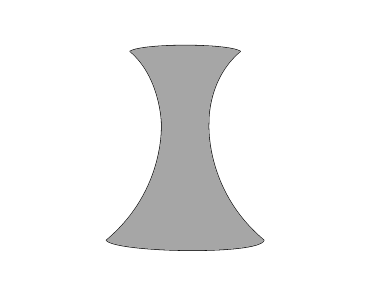
\begin{tikzpicture}[line join=round, line cap=round,scale=1,transform shape]
		\clip (-2,-1.5) rectangle (2,1.5);
		\tikzset{thap/.pic={
				\def\D{ 
					(-.7,1.2)
					..controls +(-40:.5) and +(110:0) .. (-.3,.3)%ok
					..controls +(-120:0) and +(40:1) .. (-1,-1.2)%ok
					..controls +(-50:0.2) and +(-110:0.2) .. (1,-1.2)
					..controls +(140:1) and +(-40:0) .. (.3,.3)
					..controls +(45:0) and +(-140:.55) .. (.7,1.2)
					..controls +(150:0.2) and +(30:0.2) .. (-.7,1.2)
					;}
				\draw \D;
				\fill[gray!70!] \D;
		}}
		\path(0,0)pic[scale=1]{thap};
	\end{tikzpicture}
}
\loigiai{
\immini{
Ta có
\begin{itemize}
	\item Độ dài nửa trục thực bằng $30\,\textrm{m}$ nên $a=30$.
	\item Độ dài nửa trục ảo bằng $50\,\textrm{m}$ nên $b=50$.
\end{itemize}
Phương trình chính tắc của Hypebol là
\begin{equation*}
	(H)\colon\dfrac{x^2}{30^2}-\dfrac{y^2}{50^2}=1.
\end{equation*}
}{
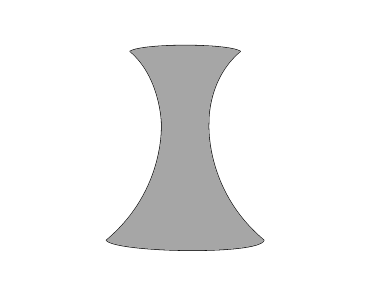
\begin{tikzpicture}[line join=round, line cap=round,scale=1,transform shape]
	\clip (-2,-1.5) rectangle (2,1.5);
	\tikzset{thap/.pic={
			\def\D{ 
				(-.7,1.2)
				..controls +(-40:.5) and +(110:0) .. (-.3,.3)%ok
				..controls +(-120:0) and +(40:1) .. (-1,-1.2)%ok
				..controls +(-50:0.2) and +(-110:0.2) .. (1,-1.2)
				..controls +(140:1) and +(-40:0) .. (.3,.3)
				..controls +(45:0) and +(-140:.55) .. (.7,1.2)
				..controls +(150:0.2) and +(30:0.2) .. (-.7,1.2)
				;}
			\draw \D;
			\fill[gray!70!] \D;
	}}
	\path(0,0)pic[scale=1]{thap};
\end{tikzpicture}
}
Gọi khoảng cách từ nóc tháp đến tâm đối xứng của Hypebol là $h$ thì khoảng cách từ tâm đối xứng đến đáy là $2h$.\\
Khi đó, chiều cao của tháp là $h+2h=3h$.\\
Mà chiều cao của tháp là $120\textrm{m}$ nên ta có
\begin{equation*}
	3h=120\Leftrightarrow h=40\,\textrm{m}.
\end{equation*}
Suy ra
\begin{equation*}
	\dfrac{x^2}{30^2}-\dfrac{80^2}{50^2}=1\Rightarrow x\approx 36{,}6\,\textrm{m}.
\end{equation*}
}
\end{bt}




